\documentclass{article}
\usepackage[margin=1in]{geometry}
\usepackage{amsmath,amsfonts,amssymb}
\usepackage{multicol}
\usepackage{graphicx}
%\usepackage{nopageno}
\usepackage{fancyhdr}
\pagestyle{fancy}
\lhead{Applied Physics}
\rhead{Page No. \thepage}
\cfoot{\textit{This document has been compiled by physics staff for private circulation in VCET, solely for the benefit of students. Permission is granted to use and distribute this material strictly for non-commercial purposes. Some content has been referenced from various academic sources, and all rights remain with the original copyright holders.}}
\renewcommand{\headrulewidth}{0.4pt}
\renewcommand{\footrulewidth}{0.4pt}

\usepackage{array}
\usepackage{booktabs}
\usepackage{tabularx}
\renewcommand{\arraystretch}{1.3} % Adjust row spacing

\usepackage[final]{pdfpages}
\usepackage{fancyhdr, blindtext}
\usepackage{afterpage}


\begin{document}


\begin{center}
\begin{minipage}{0.1\textwidth}

\includegraphics[scale=0.1]{vcet-logo.jpeg}
\end{minipage}
 \hfill 
\begin{minipage}{0.85\textwidth}
 \textbf{\Large \textbf{\begin{center}  Vidyavardhini's College of Engineering and Technology, Vasai (West) \end{center} }}
\end{minipage}

\vspace{0.3cm}
\textbf{\Large \underline{First Year Engineering}} \\
\vspace{0.5cm}
\textbf{\large Academic Year: 2024$-$2025 (NEP Syllabus) } \\
\end{center}

\noindent
%\textbf{Academic Year: 2024-2025} \hfill { \textbf{Date: 20/11/2024} }\\
%\textbf{Max Marks: 10} \hfill { \textbf{Duration: 1 Hr} }\\
\hrule
\begin{center}
\textbf{\Large Applied Physics (PYQ)} 
\end{center}
\hrule
\vspace{0.3cm}

%\begin{center} \textbf{ \Large \underline{Course Objectives}} \end{center}

%\begin{tabularx}{\textwidth}{|c|X|}
%	\hline
%	\textbf{1} & To provide students with a basic understanding of laser operation. \\
%	\hline
%	\textbf{2} & To explain the basic working principle of optical fiber and its use in communication technology. \\
%	\hline
%	\textbf{3} & To demonstrate principles of interference in thin film. \\
%	\hline
%	\textbf{4} & To describe Maxwell's equations and their significance. \\
%	\hline
%	\textbf{5} & To build a foundation of quantum mechanics needed for modern technology. \\
%	\hline
%	\textbf{6} & To give exposure to the concept of Fermi level in semiconductors. \\
%	\hline
%\end{tabularx}
%
%\vspace{1cm}

\begin{center} \textbf{ \Large \underline{Course Outcomes}} \end{center}


\vspace{0.5cm}
\begin{center}
\hrule
\vspace{0.5cm}
\textbf{ \large CO1: Illustrate the use of laser in LiDAR and Barcode reading } 
\vspace{0.5cm}

\hrule

\vspace{0.5cm}
\textbf{ \large CO2: Apply the foundation of fiber optics in the development of modern communication technology } 
\vspace{0.5cm}

\hrule

\vspace{0.5cm}
\textbf{ \large CO3: Determine the wavelength of light and refractive index of liquid using the interference phenomenon} 
\vspace{0.5cm}

\hrule

\vspace{0.5cm}
\textbf{ \large CO4: Illustrate the significance of Maxwell's equations in the field of modern technology} 
\vspace{0.5cm}

\hrule

\vspace{0.5cm}
\textbf{ \large CO5: Apply the foundations of quantum mechanics for the development of modern technology} 
\vspace{0.5cm}

\hrule

\vspace{0.5cm}
\textbf{  \large CO6: Explain the types of semiconductors based on variations in Fermi level with temperature and doping concentration} 
\vspace{0.5cm}
\hrule
\end{center}

\vspace{1.5cm}

\textit{In physics, you don't have to go around making trouble for yourself, nature does it for you. Nothing in life is to be feared, it is only to be understood.  Now is the time to understand more, so that we may fear less.}  \hfil $-$ \textit{Frank Wilczek \& Allan Sandage}

\textit{
}

%\begin{tabularx}{\textwidth}{|c|X|c|c|}
%	\hline
%	\textbf{Code} & \textbf{ \centering At the end of the course, students will be able to:} & \textbf{Action Verb} & \textbf{Bloom's Level} \\
%	\hline
%	BSC102.1 & Illustrate the use of laser in LiDAR and Barcode reading. & Illustrate & Level 3 \\
%	\hline
%	BSC102.2 & Apply the foundation of fiber optics in the development of modern communication technology. & Apply & Level 3 \\
%	\hline
%	BSC102.3 & Determine the wavelength of light and refractive index of liquid using the interference phenomenon. & Determine & Level 3 \\
%	\hline
%	BSC102.4 & Illustrate the significance of Maxwell's equations in the field of modern technology. & Illustrate & Level 3 \\
%	\hline
%	BSC102.5 & Apply the foundations of quantum mechanics for the development of modern technology. & Relate & Level 3 \\
%	\hline
%	BSC102.6 & Explain the types of semiconductors based on variations in Fermi level with temperature and doping concentration. & Explain & Level 3 \\
%	\hline
%\end{tabularx}

\newpage

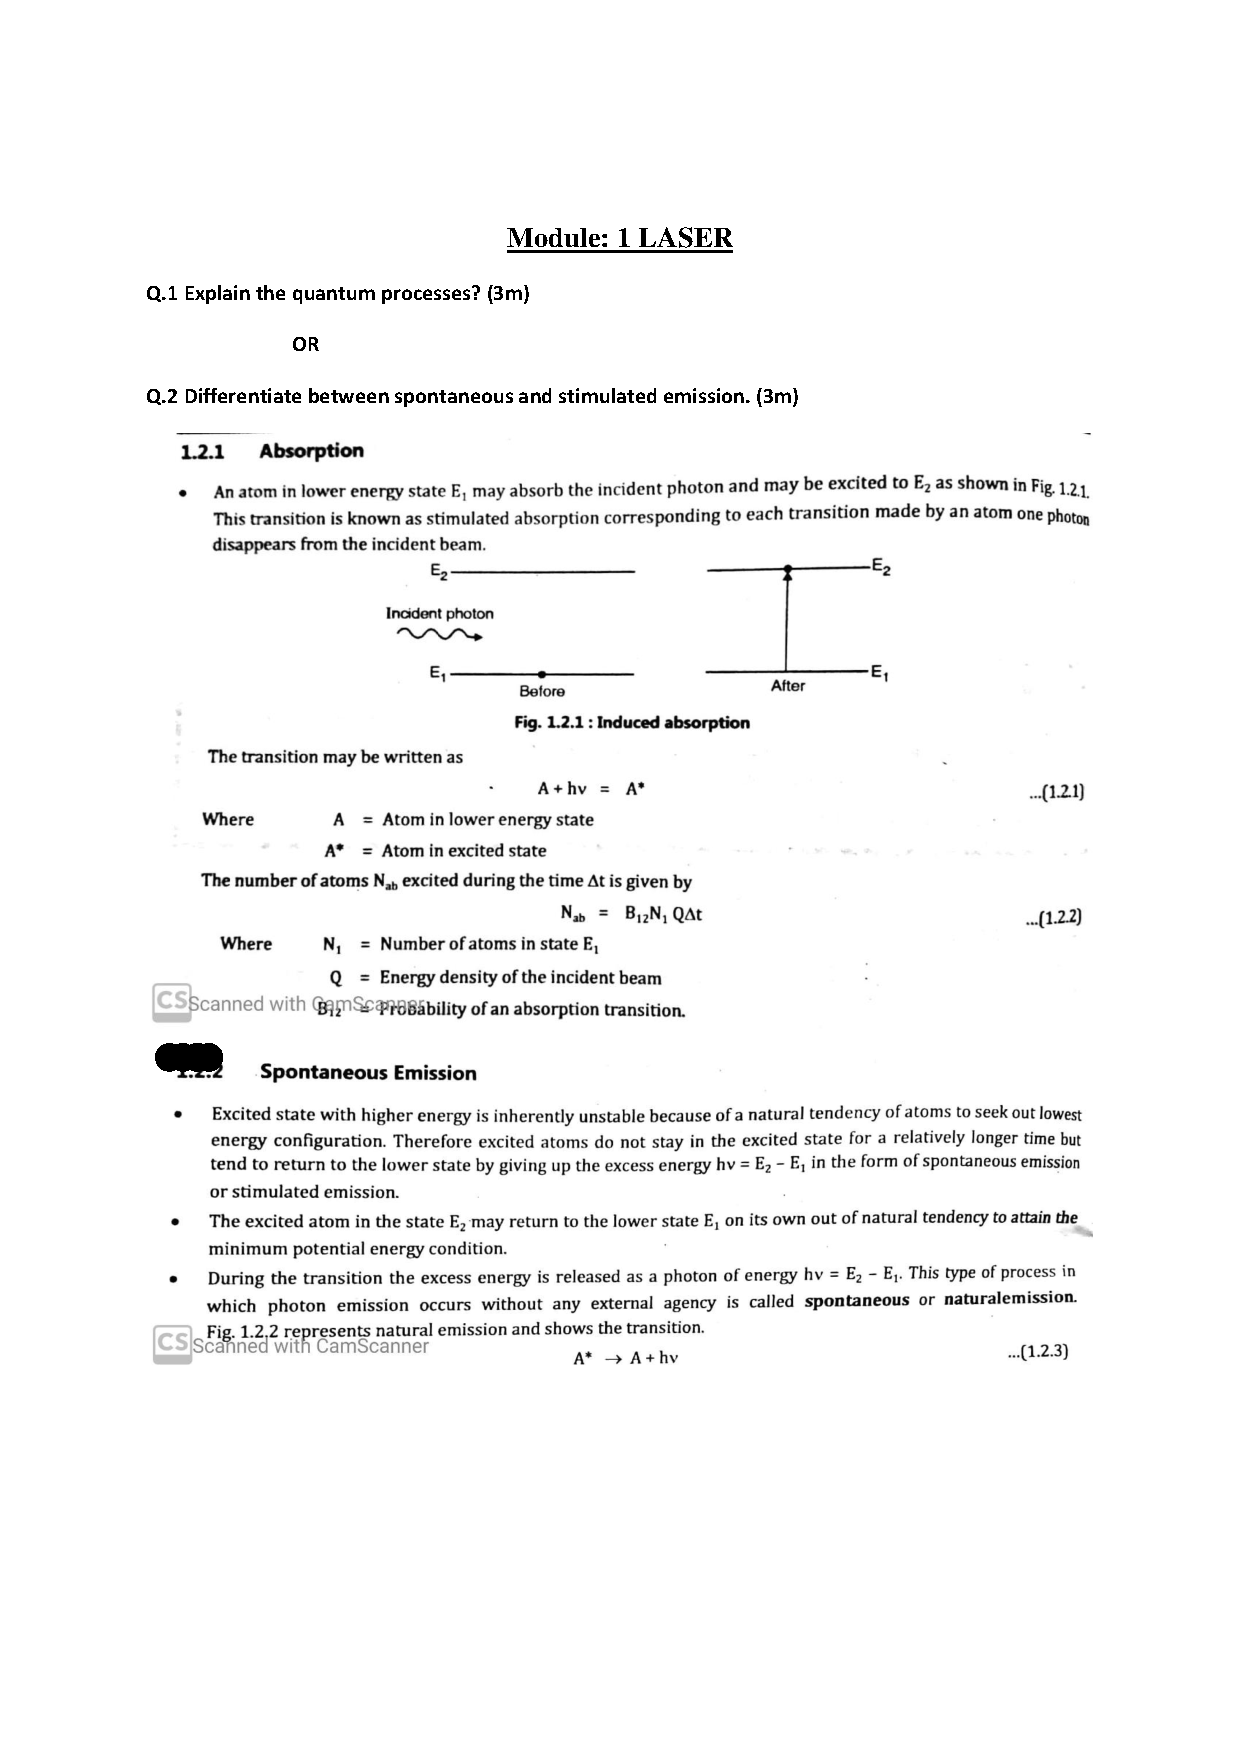
\includepdf[pages=-,pagecommand={\thispagestyle{fancy}},offset=0mm 0mm]{Mod-1.pdf}
%
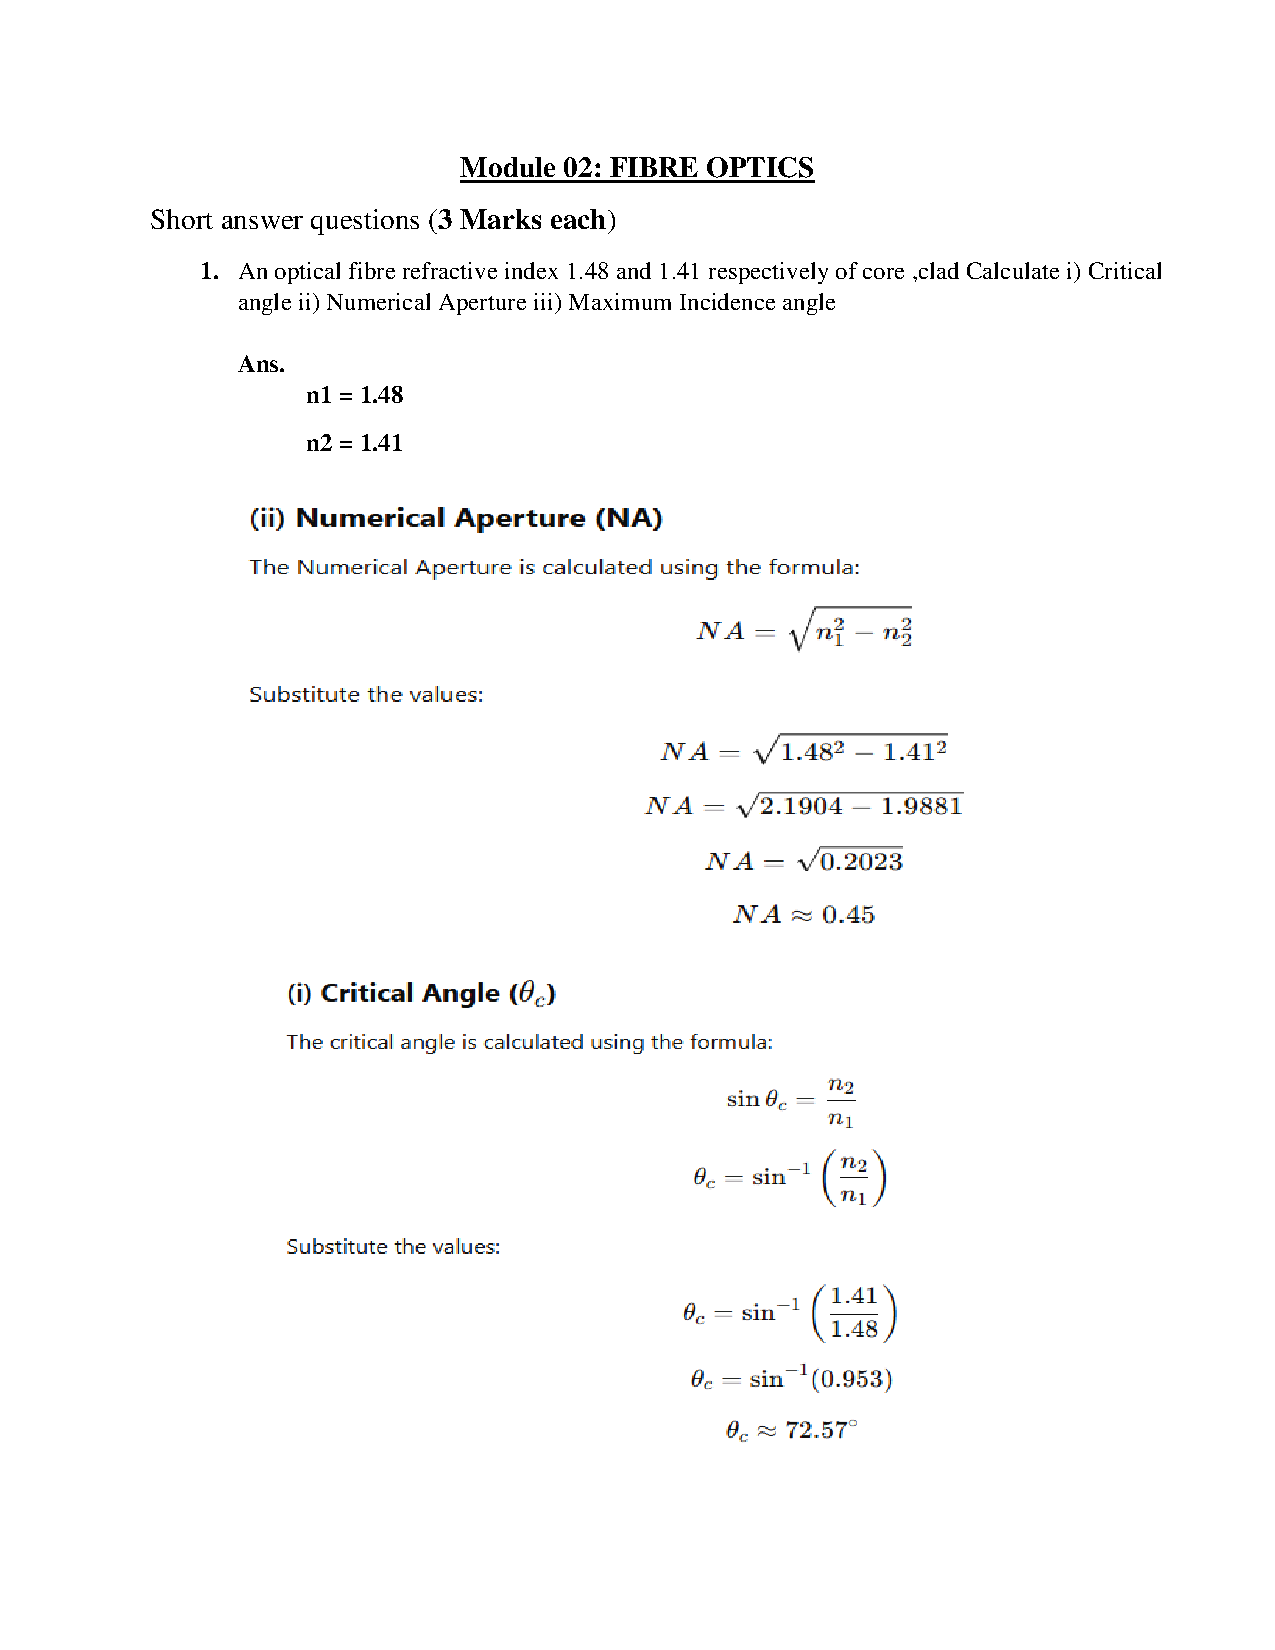
\includepdf[pages=-,pagecommand={\thispagestyle{fancy}},offset=0mm 0mm]{Mod-2and3.pdf}
%
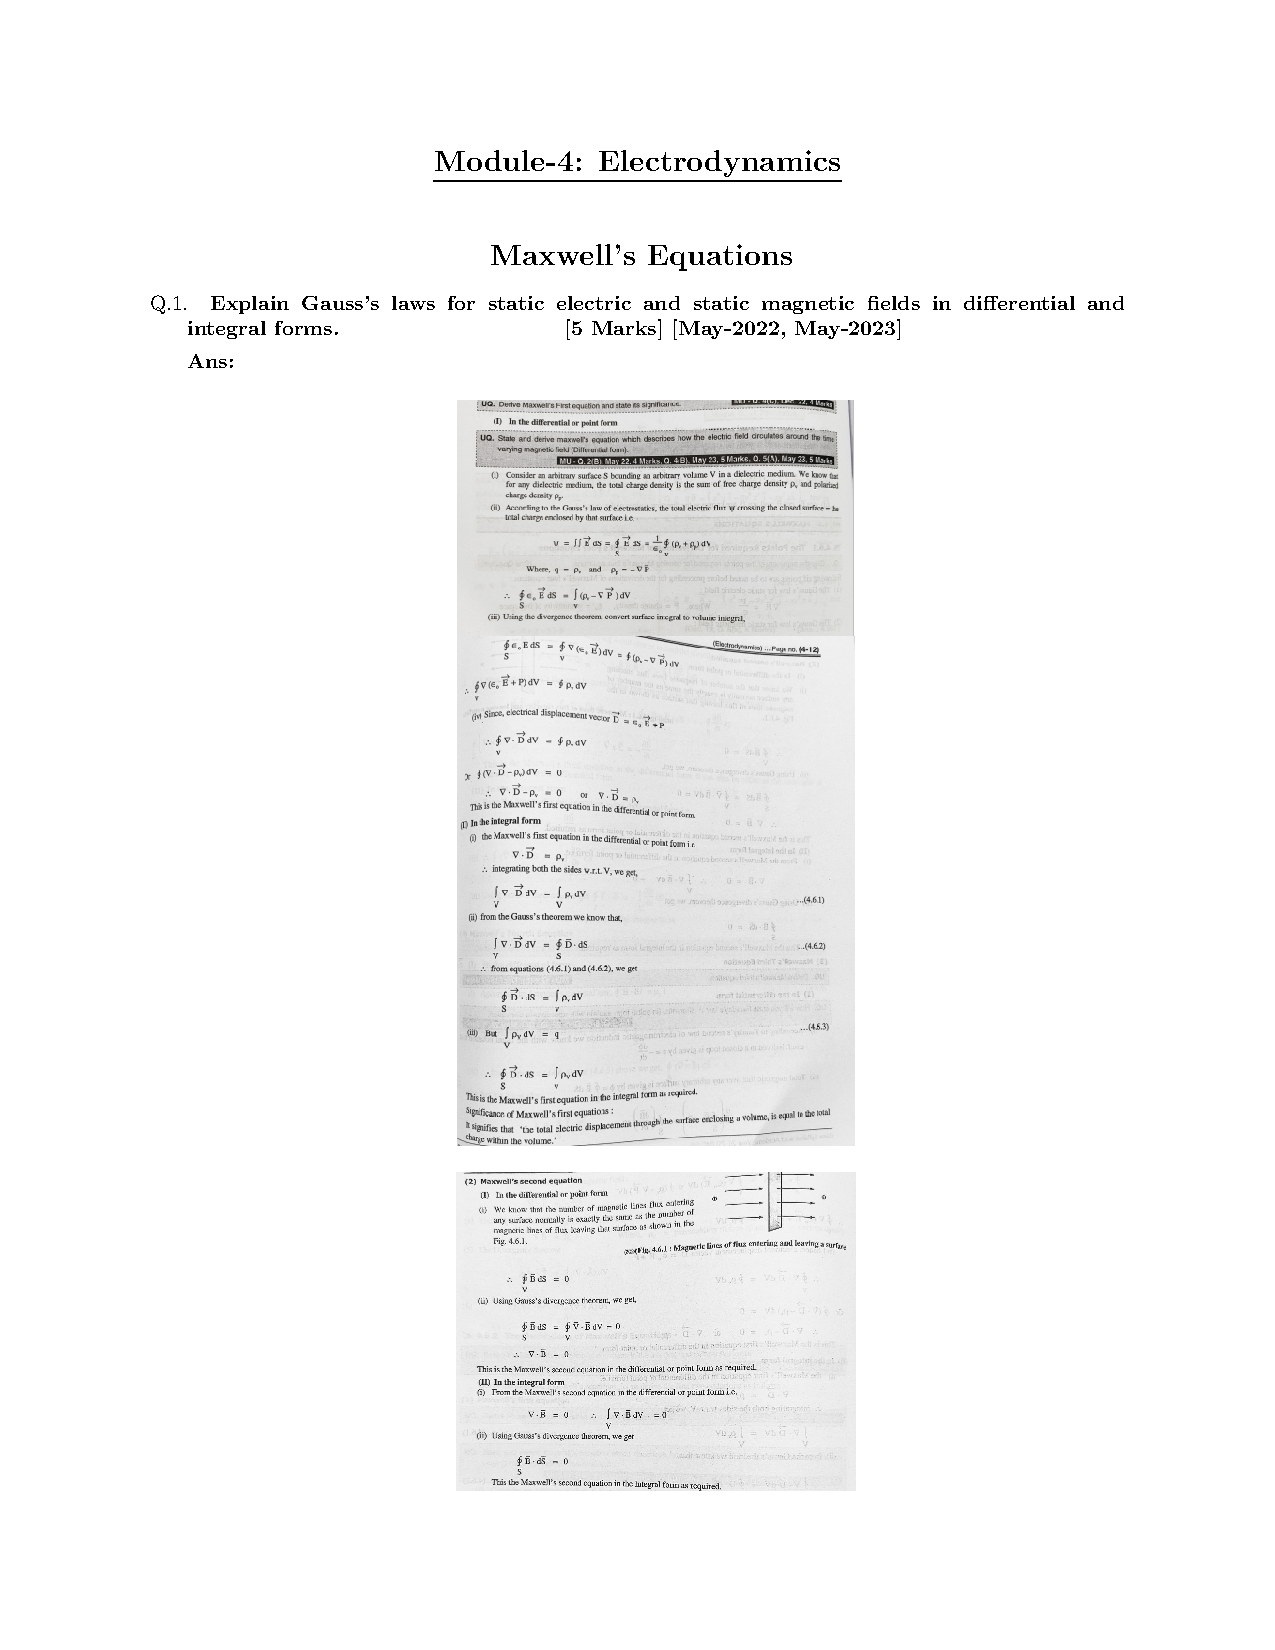
\includepdf[pages=-,pagecommand={\thispagestyle{fancy}},offset=0mm 0mm]{Mod-4.pdf}
%
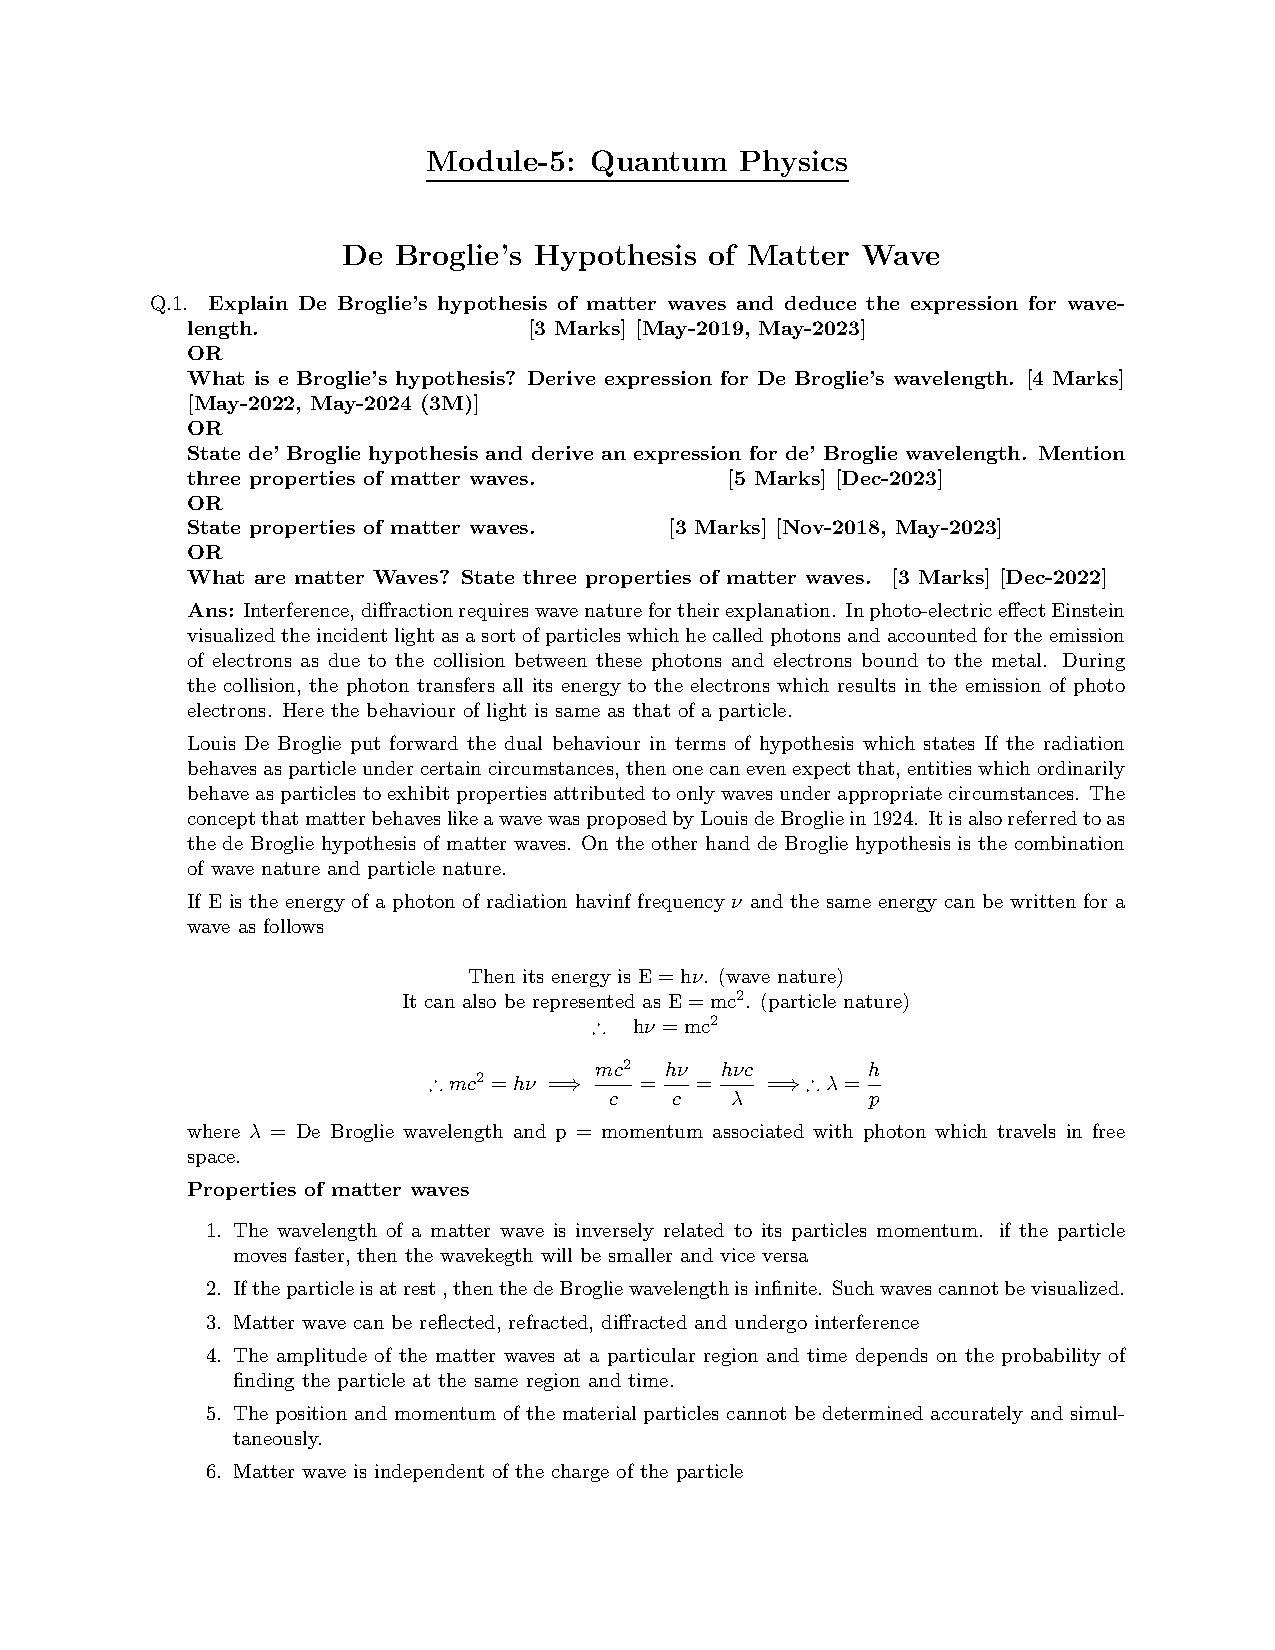
\includepdf[pages=-,pagecommand={\thispagestyle{fancy}},offset=0mm 0mm]{Mod-5.pdf}
%
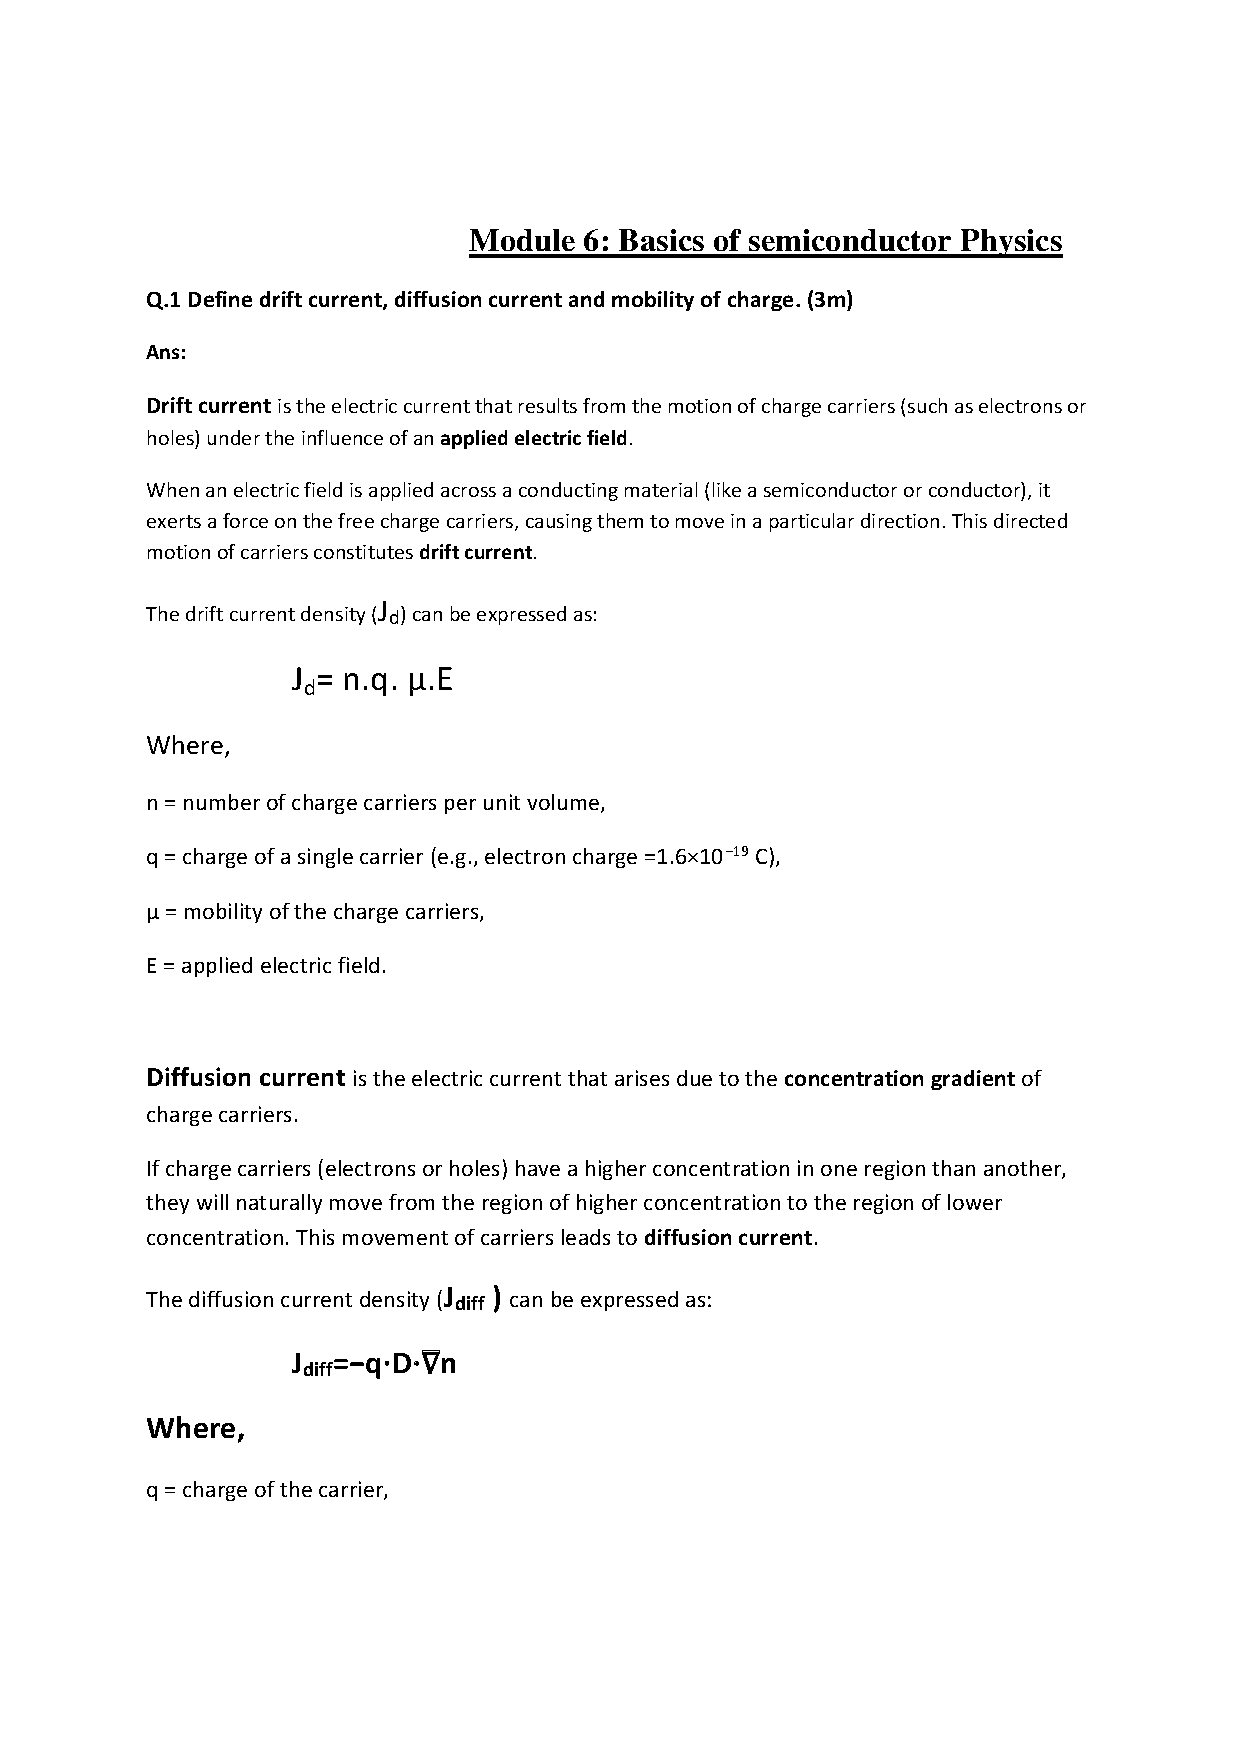
\includepdf[pages=-,pagecommand={\thispagestyle{fancy}},offset=0mm 0mm]{Mod-6.pdf}

\end{document}
